\documentclass[12pt]{article}
\author{Martin Ludvigsen}
\title{TMA4280 - Project 1}

\usepackage{amsmath}
\usepackage{graphicx}
\graphicspath{{figures/}}

\begin{document}
\maketitle
\section{Introduction}
The project was written in Fortran, using a home-brewed Makefile and Python for plotting. The organization of the folders
should make it obvious where the files are located. The project can be downloaded from github using this link:
\begin{equation*}
    \texttt{https://github.com/martilud/TMA4280project1.git}
\end{equation*}
Throughout the entire project, i used \texttt{REAL} instead of \texttt{DOUBLE PRECISION} variables, and used compiler flags to ensure double precision for both floats and integers.
This was somewhat inconsistent, as i had to use \texttt{MPI\_DOUBLE\_PRECISION} instead of \texttt{MPI\_REAL} later.

The objective of the project is to calculate $\pi$ using two formulae, rewritten slightly from the problem description. First, the simple, yet beautiful Riemann-Zeta/Basel problem formula
first proved by Euler:
\begin{equation}
    \lim_{n \rightarrow \infty} \sum_{i = 1}^n \frac{1}{i^2} = \frac{\pi^2}{6},
    \label{eq:zeta}
\end{equation}
and secondly, the slightly more complex, "original" Machin formula, based on the Taylor series expansion of $\text{arctan} x$:
\begin{equation}
    \lim_{n \rightarrow \infty} \sum_{i = 1}^n (-1)^{i-1} \frac{1}{2i-1}\left(4 \left(\frac{1}{5}\right)^{2i-1} - \left(\frac{1}{239}\right)^{2i-1}\right) = \frac{\pi}{4}.
    \label{eq:mach}
\end{equation}

\section{Question 1. Serial Implementation}
In both formulae, we can expect roundoff errors for large $i$. In double precision, the mantissa uses $52$ bits, meaning the smallest "distance" we can measure
between numbers is $2^{-52} \approx 2.22 \times 10^{-16}$. This also means that the order of operations in our calculations actually matter, as floating point operations are not commutative.
Note that for \eqref{eq:mach}, it's much faster to calculate $\left(\frac{1}{5}\right)^{2i-1}$ by saving $\left(\frac{1}{5}\right)$ in a variable and multiplying it by 
$\left(\frac{1}{5}\right)^2$ each iteration instead of calculating it bottom up each iteration.
My implementation showed to be sufficiently numerically stable, as we will see later. 

\section{Question 2. Unit Test(s)}
A unit test is a fast test of our program. The purpose of a 
unit test is to check the logic in our code to ensure it runs correctly.
In larger programs, one usually runs unit tests on small parts of code
to ensure that every part works as intended. In our toy example, we only
have to check if the program actually runs, and returns something slightly logical.
For this, I could have written a separate Fortran program, bash script of some sort or used some unit testing software.

But before we write anything, what whould we test to ensure our code works correctly? For \eqref{eq:zeta}, we see that a partial sum will always be (up to floating point errors), between $1$ and
$\frac{\pi^2}{6}$. Thus we can check if the error in our calculated $\pi_n$, calculated as $|\pi - \pi_n|$, is somewhere between $1$ and $\pi - \sqrt{6}$.

Using similar logic for \eqref{eq:mach}
we see that the first term in the sum is $\frac{4}{5} - \frac{1}{239}$, and all subsequences should be closer to $\pi$ than this by the error bound provided by the
alternating series test (REFERANSE). Thus, we can check if the error is larger than $4 *(\frac{4}{5} - \frac{1}{239}) - \pi$, as no subsequence should have a higher error than this.  

When implementing, it proved to be simplest to just program the test into our original program, and use the command line to input if we want to test. This was mostly because bash scripts can't
handle floating point numbers and i did not want to bother linking different Fortran scripts together. The simplest solution is often the best solution.

We can then make a command in the Makefile to execute our unit test(s) easily, either by typing for example \texttt{make zeta0utest} to run the \texttt{zeta0} unit test or
\texttt{make utest} to run all unit tests. Figure \ref{fig:Q2} shows the output of our unit test(s). It works! 
\begin{figure}[!htb]
    \centering
    \caption{Result of running \texttt{make utest}}
    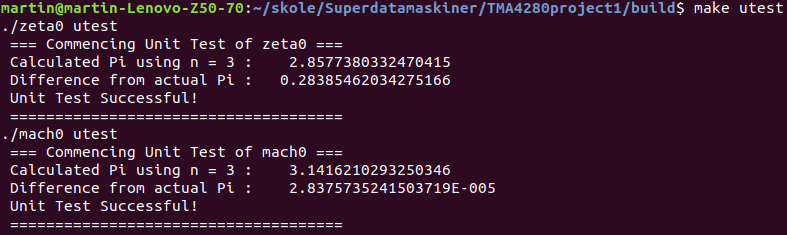
\includegraphics[width=\textwidth]{Screenshot2}
    \label{fig:Q2}
\end{figure}

\section{Question 3. Verification Test(s)}
Now that we know our programs work, we have to see if the mathematics behave nicely. For simplicity, this was also programmed directly into our existing program similarily to the Unit Test.
In our verification test, we check the error for many different $n$, and save the resulting error and the time it took calculate in a textfile. This can be executed similarily
to the unit test, just swap the word \texttt{utest} with \texttt{vtest}.

Results from running the verification tests are shown in figures \ref{fig:Convergence1} and \ref{fig:Time1}. 

\begin{figure}[!htb]
    \centering
    \caption{Convergence result of running \texttt{make vtest}}
    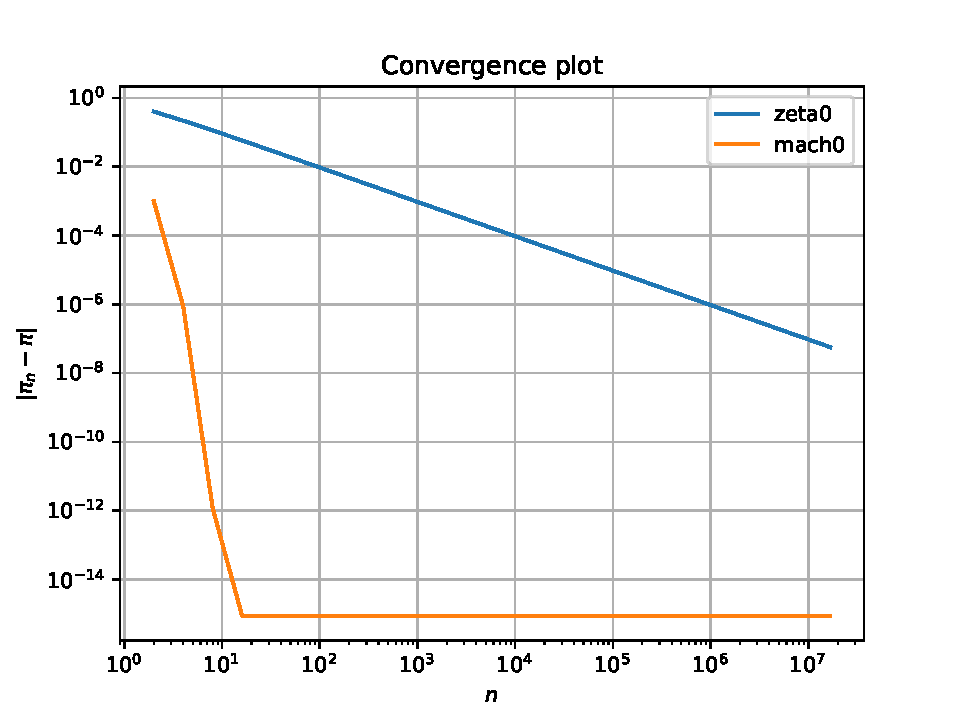
\includegraphics[width=\textwidth]{Convergence1}
    \label{fig:Convergence1}
\end{figure}

\begin{figure}[!htb]
    \centering
    \caption{Timing result of running \texttt{make vtest}}
    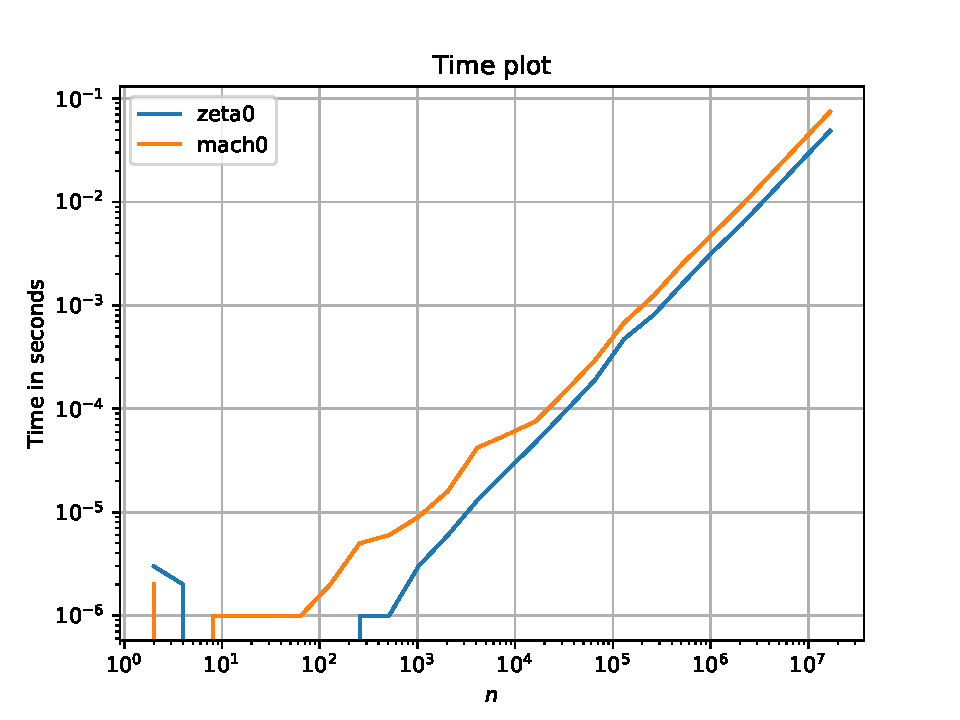
\includegraphics[width=\textwidth]{Time1}
    \label{fig:Time1}
\end{figure}
We see that the Machin formula quickly converges to 

\section{References}
FIXX ME
https://en.wikipedia.org/wiki/Alternating\_series\_test
\end{document}
